% This must be in the first 5 lines to tell arXiv to use pdfLaTeX, which is strongly recommended.
\pdfoutput=1
% In particular, the hyperref package requires pdfLaTeX in order to break URLs across lines.

\documentclass[11pt]{article}

% Remove the "review" option to generate the final version.
\usepackage{acl}

% Standard package includes
\usepackage{times}
\usepackage{latexsym}

% For proper rendering and hyphenation of words containing Latin characters (including in bib files)
\usepackage[T1]{fontenc}
% For Vietnamese characters
% \usepackage[T5]{fontenc}
% See https://www.latex-project.org/help/documentation/encguide.pdf for other character sets

% This assumes your files are encoded as UTF8
\usepackage[utf8]{inputenc}

% This is not strictly necessary, and may be commented out,
% but it will improve the layout of the manuscript,
% and will typically save some space.
\usepackage{microtype}

\usepackage{graphicx}
\usepackage{cleveref}

% If the title and author information does not fit in the area allocated, uncomment the following
%
%\setlength\titlebox{<dim>}
%
% and set <dim> to something 5cm or larger.

\title{Homework 1}
\author{Pedro Matias \\
  \texttt{pmatias@uci.edu}}

\begin{document}
\maketitle
\section{Preliminaries}\label{sec:prelim}

A basic data analysis, summarized in \cref{fig:dataset}, showed that the dataset is unbalanced when it comes to total number of documents/words/letters, where higher numbers of these correlate with democrat affiliation. The average number of words per document, letters per document and letters per word is pretty identical across across the candidates. Indeed, initial experiments showed that assigning weights inversely proportional to each label frequency results (more often than not) in better accuracies, so we adopted this strategy throughout our experiments. During these initial experiments, we gained further information that made us adopt the following strategies in later experiments:

\begin{itemize}
  \item using 5-fold \textbf{cross-validation}, scored using the accuracy averaged across folds, since the small labeled-to-unlabeled ratio could promote overfitting. We used \textit{stratified} folds to promote even label frequencies (since data is unbalanced). We also merged train and dev data for this purpose.
  \item using \textbf{TF-IDF}, as opposed to bag-of-words (counting or binary) model
  \item using both word-unigrams and \textbf{word-bigrams}, as opposed to just word-unigrams. In our case, the dependencies between consecutive words modeled by bigrams features helped the results slightly. We did not have time to try character n-grams
  \item using \texttt{nltk.word\_tokenize} on \textbf{lowercase} text, as opposed to \texttt{Scikit-learn}'s default tokenizer
  \item not removing \textbf{stopwords}, since early experiments did not make worthy improvements, but also because we (i) used TD-IDF (which already discounts words with high document-frequencies), but also (ii) entirely removed words with high document-frequencies cutoffs (see \cref{sec:super})
  \item using L2-regularization, as opposed to L1, given early experiment results
  \item using a maximum of 100 \textbf{iterations} for Logistic Regression convergence, as opposed to larger values (which did not increase the cross-validation accuracy and were slower) or smaller values (for which we underfit). When combining TF-IDF with other features (see \cref{sec:semi}), we used larger values to avoid underfitting.
\end{itemize}



\begin{figure}
  \centering
  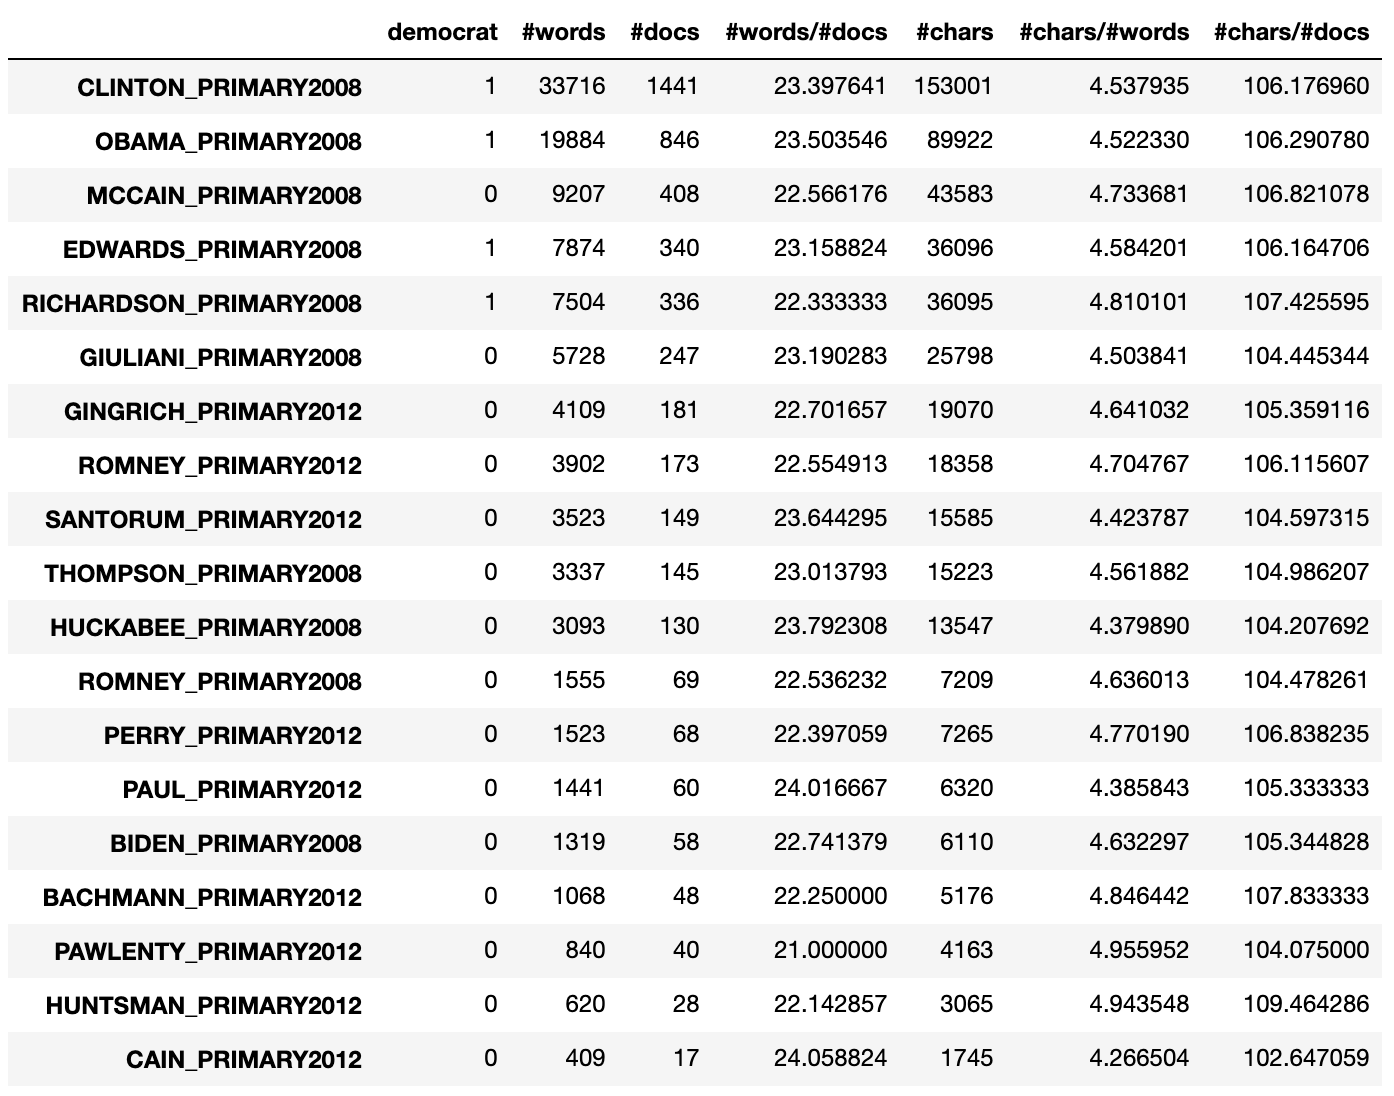
\includegraphics[height=3in]{figures/stats.png}
  \caption{Dataset analysis.}
  \label{fig:dataset}
\end{figure}


\section{Supervised}\label{sec:super}

We experimented with different configurations and noticed an increase in accuracies for higher values of $C$, the inverse of regularization strength, as depicted in \cref{fig:supervised}. It is interesting to note that changes in accuracy caused by varying document-frequencies cutoffs (i.e. the minimum document-frequency of a word considered for removal) was only noticeable for larger values of $C$, where accuracies were higher for higher cutoffs (i.e. less words were removed). A possible explanation is the fact that the stratregy of assigning higher weights (give less regularization) to words works best when the vocabulary size considered is indeed higher.

Indeed, increasing $C$ even further resulted in even better results, until $C$ assumes values bigger than 100, at which point the accuracy starts decreasing. Our best configuration, with respective accuracy scores was the following (see \cref{sec:prelim} for the remaining hyperparams setting):

\begin{center}
\begin{tabular}{r|c}
  $\mathbf{C}$ & 80 \\\hline 
  \textbf{frequency cutoff} & 0.9 \\\hline
  \textbf{train accuracy} & 0.999 \\\hline
  \textbf{cross-validation accuracy} & 0.464 \\\hline
  \textbf{Kaggle accuracy}  & 0.491
\end{tabular}
\end{center}


\begin{figure}
\centering
  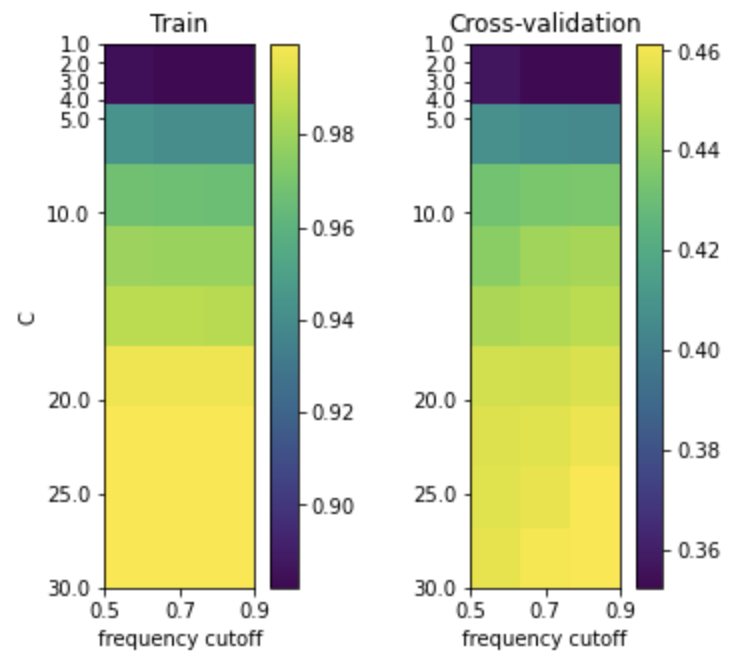
\includegraphics[width=3in]{figures/supervised.png}
  \caption{Varying document-frequency cutoff for removing words (x-axis) against regularization levels (y-axis) for Logistic Regression (higher values of $C$ correspond to less regularization). See \cref{sec:prelim} for remaining hyperparams configuration.}
  \label{fig:supervised}
\end{figure}

\section{Semi-supervised}\label{sec:semi}

We tried incorporating word2vec embeddings, using Gensim's implementation. We generated these embeddings by training on both the labeled and unlabeled data provided. We also tried GloVe's pre-computed word2vec embeddings (Wikipedia 2014 + Gigaword 5, for 50-dimension), but results didn't differ significantly from results given by embeddings trained on the corpus itself. To combine the embeddings of each word in a single document, we tried the following approaches, while varying the number of dimensions (100, 150, 200) and the context window sizes (5, 10, 15, 20) (see \cref{fig:acc_embeddings}):

\begin{itemize}
  \item Coordinate-wise \textbf{average} of all embeddings in the document
  \item Coordinate-wise \textbf{TF-IDF weighted average} of all embeddings in the document
  \item Coordinate-wise \textbf{sum} of all embeddings in the document
  \item Coordinate-wise \textbf{minimum} and/or \textbf{maximum} of all embeddings in the document
\end{itemize}

\begin{figure}
\centering
  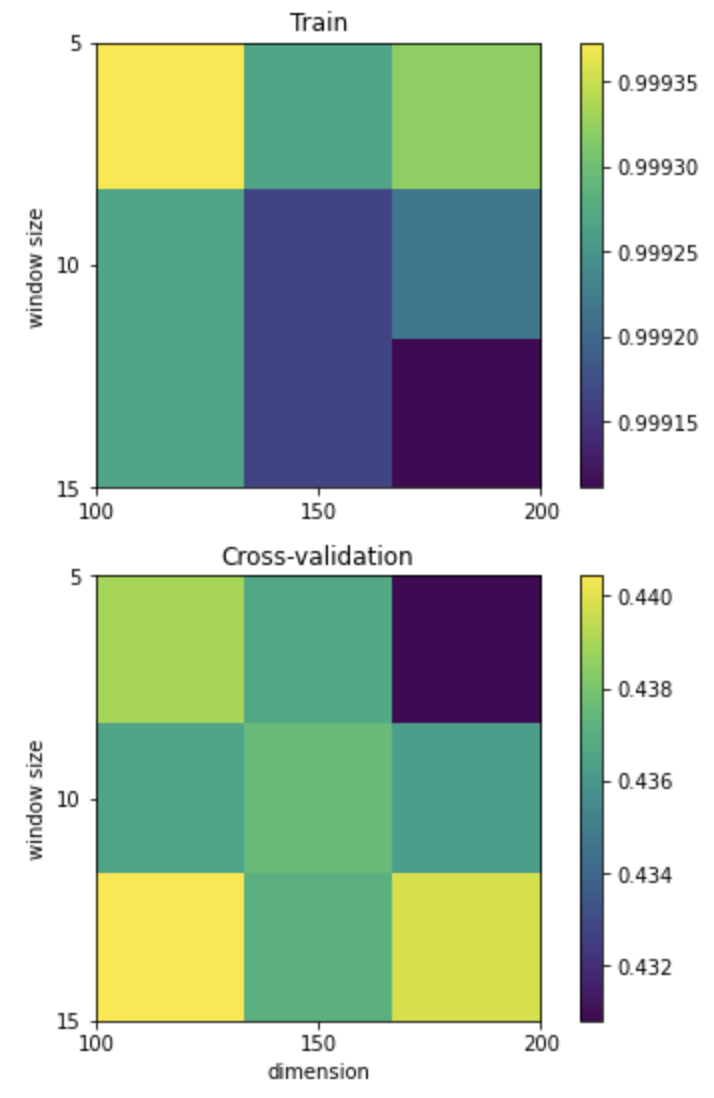
\includegraphics[width=2in]{figures/embeddings_windows_dims.png}
  \caption{Accuracy varying context window sizes and output embedding dimensions.}
  \label{fig:acc_embeddings}
\end{figure}

The best type of aggregation was TF-IDF weighted average. Close to this was regular average. The remaining types of aggregation had very small accuracies (less than half).

Unfortunately, we were not able to find a good configuration of hyperparams for TF-IDF weighted average, and our best model delivered the following accuracies (we increased the number of iterations from 100, since the increased number of features requires more time to avoid underfitting):

\begin{center}
\begin{tabular}{r|c}
  $\mathbf{C}$ & 95 \\\hline 
  \textbf{frequency cutoff} & 0.9 \\\hline
  \textbf{\#iterations} & 200 \\\hline
  \textbf{w2v aggregation} & TF-IDF weighted avg. \\\hline 
  \textbf{train accuracy} & 0.999 \\\hline
  \textbf{cross-validation accuracy} & 0.453 \\\hline
  \textbf{Kaggle accuracy}  & 0.476
\end{tabular}
\end{center}

Indeed, the embeddings produced are not representative of each presidential candidate -- see \cref{fig:labeled_centroids} for a comparison between the average embedding for each presidential candidate.

\subsection{Clustering}\label{subsec:clustering}

Next, we tried the following approach:

\begin{enumerate}
  \item use a \textbf{clustering} technique to cluster the union of labeled (train+dev) and unlabeled data, into $K$ clusters
  \item determine a \textbf{mapping} between clusters and presidential candidates, using the labeled data. This mapping can be one-to-one, one-to-many or even many-to-one, depending on $K$
  \item label the unlabeled data according to the previous mapping 
  \item re-train the previous best supervised classifier using both the initial labels and the ones generated in the previous step
\end{enumerate}

To perform clustering, we resorted to lower-dimensional word2vec embeddings, using Gensim implementation. As in the previous section, we generated these by training on both the labeled and unlabeled data provided.

Before implementing the idea above mentioned, we examined the quality of embeddings produced by our supervised classifier, in the sense of how good they cluster the labeled data -- see \cref{fig:labeled_centroids} for details. As illustrated, the average embeddings for each candidate are very similar to each other, suggesting that labeled ``clusters'' are overlapping quite a bit, yielding bad representative embeddings. The similarity between candidates seems even more pronounced when comparing using cosine similarity and this may be due to the fact that it ignores vectors norms.

\begin{figure}[t]
  \label{fig:labeled_centroids}
\centering
  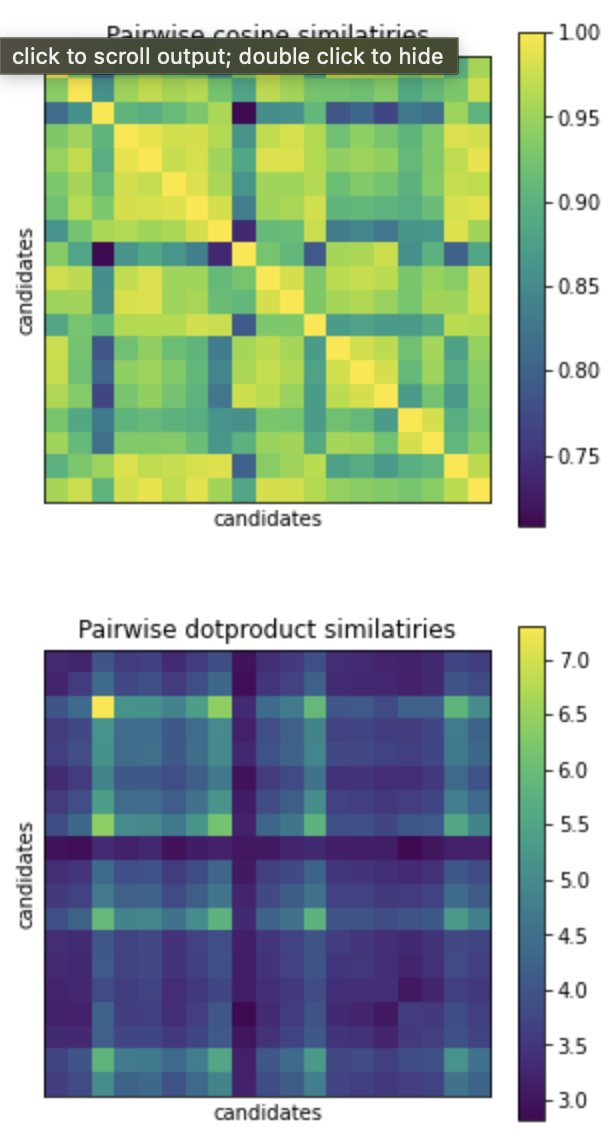
\includegraphics[width=2.5in]{figures/word2vecs.png}
  \caption{Similarities between the average (a.k.a. centroid) embedding for each presidential candidate, suggest that embeddings are not very representative of each candidate. The embeddings have dimension 200, were produced using a context window of size 20 and were combined using TF-IDF weighted average (other kinds of aggregations with lower dimensions/windows had similar or worse results).}
\end{figure}

To evaluate the quality of our clusterings (using K-Means and Gaussian Mixture Model (GMM)), we estimated the likelihood that the average candidate belongs to each of the clusters generated -- see \cref{fig:gmm_kmeans} for details. Particularly, we computed the probabilities $P(X_i \mid Z_j)$ that a document $X_i$ is labeled with candidate $k$, given that we know it belongs to cluster $Z_j$ and we summed these up, for each candidate $k$, to obtain $P(C_k \mid Z_j)$, which essentially models the distribution over candidates for each cluster $Z_j$. By Bayes' Rule and the assumption that $X$ follows a uniform distribution $\mathcal{U}(1,19)$, the quantities $P(X_i \mid Z_j)$ are proportional to the \emph{membership probabilities} $P(Z_j \mid X_i)$, which can be obtained directly from the weights used for K-Means/GMM. The takeaway here is that the clusters generated were not good, since they contain (with some exceptions) the same proportion of candidates. Worth noting, however, is the fact that GMM gives more representative clusters when compared to K-Means, so we used this one to retrain our supervised classifier. Unfortunately, we weren't able to find a good configuration that allowed us to improve the Kaggle accuracy obtained using the supervised classifier. It is also possible that the clusterings obtained can be improved with further fine-tuning of K-Means/GMM hyperparams, which we did not conduct due to time restrictions. Our best model is given below (see \cref{sec:prelim} for details on remaining hyperparams setting). The difference between cross-validation and Kaggle accuracies suggests overfitting occurrence.

\begin{center}
\begin{tabular}{r|c}
  $\mathbf{C}$ & 80 \\\hline 
  \textbf{frequency cutoff} & 0.9 \\\hline
  \textbf{\#iterations} & 200 \\\hline
  \textbf{train accuracy} & 0.999 \\\hline
  \textbf{cross-validation accuracy} & 0.616 \\\hline
  \textbf{Kaggle accuracy}  & 0.467
\end{tabular}
\end{center}

~

\subsubsection*{Implementation details.}

For K-Means \textbf{weights initialization}, we tried k-means++ algorithm, random initialization, and using the labeled centroids (average embedding for each candidate -- see \cref{fig:labeled_centroids}). All of these seemed to perform similarly. Regarding GMM, the parameters were initialized in a way that every mixture component has zero mean and identity covariance. The \textbf{mapping} from cluster centroids to candidates was obtained by sampling, for each cluster centroid $Z_j$, according to the probabilities $P(C_k \mid Z_j)$ computed. We avoided selecting the candidate $C_k$ with maximum presence in $Z_j$ to prevent having most clusters labeled with the most popular candidates (which tend to be democrats, see \cref{fig:dataset,fig:gmm_kmeans}). We set the number of clusters for both K-Means and GMM to $K=19$ and, for the sake of analysis, $K=2$. The latter case of $K=2$ emphasized even more the difficulty of clustering, since we obtained membership probabilities close to 50\% (i.e. $P(C_k\mid Z_1)\approx P(C_k\mid Z_2)$, for each $k$).

\begin{figure}[t]
\centering
  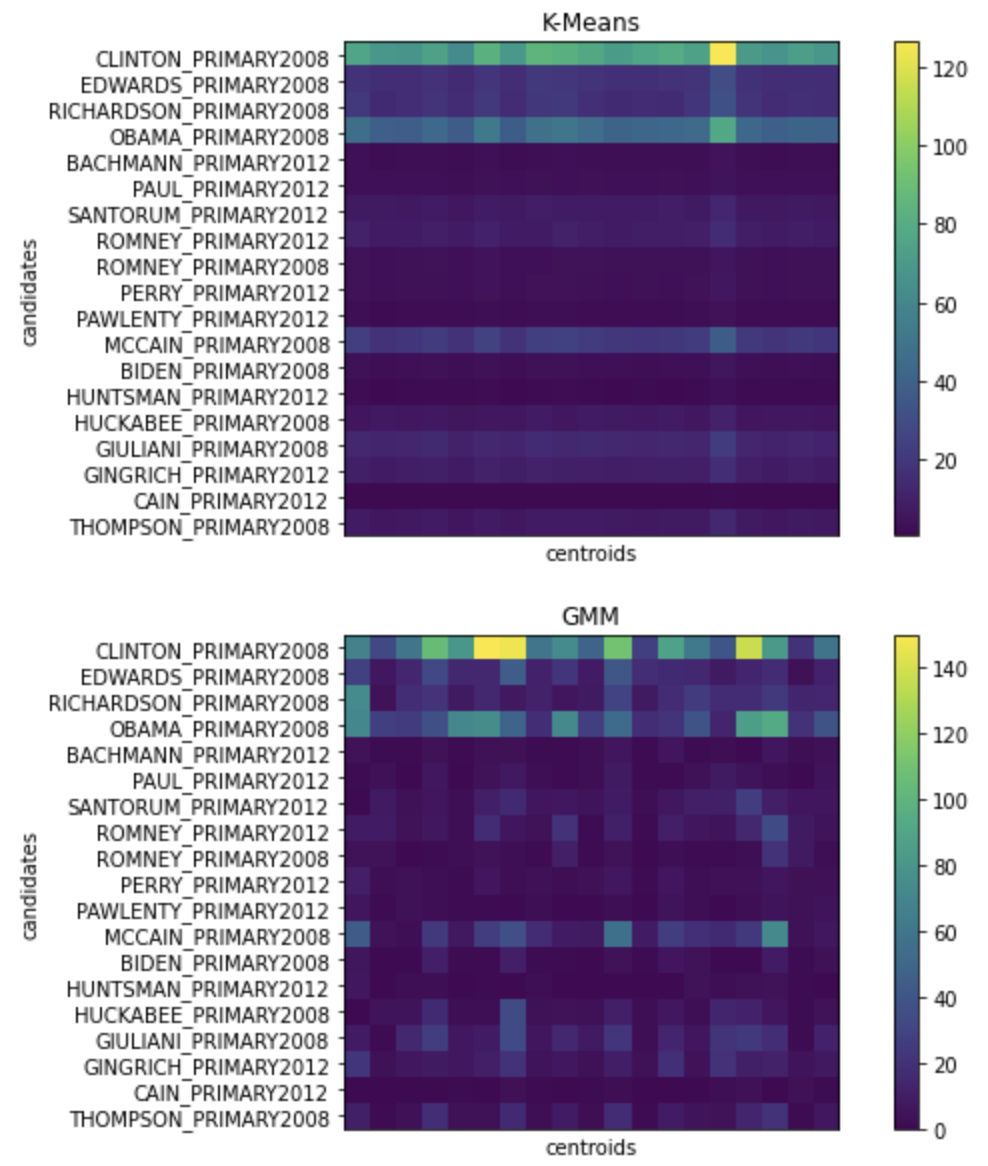
\includegraphics[width=4in]{figures/gmm_kmeans.png}
  \caption{Each row $i$ contains the membership probabilities $P(Z_j \mid C_k)$, representing the probability that the average candidate $k$ belongs to the $j$\textsuperscript{th} cluster, out of 19 clusters generated, using K-Means (initialized with k-means++) and GMM (initialized for 0 means and identity covariance). We ``joined'' the democrats together in the top-4 rows, to assess any affiliation discrepancies -- we obtained higher membership probabilities due to the unbalance in the data which favors democrats more over republicans.}
  \label{fig:gmm_kmeans}
\end{figure}

\section{Statement of collaboration}

Briefly discussed with Ramtin how to approach the semi-supervised model, namely which approach would be more interesting or more likely to work.



\end{document}
